\documentclass{article}
\usepackage[utf8]{inputenc}
\usepackage{amssymb}
\usepackage{enumitem}

\usepackage{minted}
\usepackage{xcolor}
\usemintedstyle{borland}
\definecolor{LightGray}{gray}{0.9}

\usepackage{natbib}
\usepackage{graphicx}
\usepackage{geometry}
 \geometry{
 a4paper,
 total={170mm,257mm},
 left=25mm,
 top=25mm,
 }



\title{CSE 565 - Homework 2}
\author{Amlan Gupta (\#50288686)}
\date{September 2018}


\begin{document}

\maketitle

\section {Question}

\textbf{To facilitate learning about how encryption modes work, this question asks you to derive formulas for encryption and decryption in the CFB and OFB modes. In particular, the lecture presented formulas for computing cipherblocks from plaintext and plaintext from cipherblocks for almost all modes of operation including CFB. For this question, derive similar encryption and decryption formulas for the CFB mode used as a stream cipher with r-bit messages (r $<$ n).You can use notation $S_r$(a) employed in the textbook to denote the first (most significant) r bits of a. Also use notation $\|$ to denote concatenation (i.e., a$\|$b means b appended to the end of a).\newline Repeat the exercise for the OFB mode used as a stream cipher with r-bit messages.}
\newline \newline It is possible to convert any block cipher to stream cipher using \textbf{Cipher Feedback Mode}.

\begin{figure}[h]
\centering
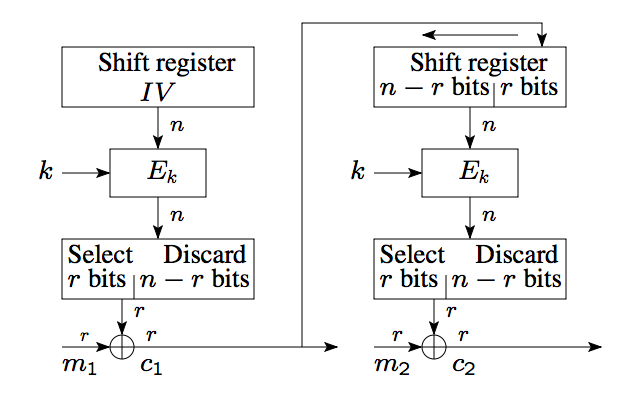
\includegraphics[scale=0.5]{cfb_encryption.png}
\caption{Encryption using Cipher Feedback Mode \citep{lecture3_marina}}
\label{fig:cfb_encryption}
\end{figure}


According to the diagram we will use a shift register, the initial value of which is set to an initialization vector IV containing n bits i.e. $I_1$ = IV
\newline \newline Then shift register will be encrypted using given key k i.e. $E_k(I_1)$
\newline \newline The left-most (most significant) r bits of the encrypted output,  $S_r(E_k(I_1))$ will be XOR-ed with r-bit plain-text $m_1$. The resulting output is ciphertext $C_1$ of length r bits.
\newline So, $C_1$ = $S_r$($E_k$($I_1$)) $\oplus$ $m_1$
\newline \newline Once $C_1$ gets generated, the contents of the shift register are left-shifted by r bits and C1 is placed in the right-most (least significant) r bits of the shift register i.e $I_2$ = $ (I_1 \ll r)  \|  C_1$
\newline \newline Generalizing this formula we get,

$C_i$ = $S_r(E_k(I_i))$ $\oplus$ $m_i$ ; $I_{i+1}$ = $ (I_i \ll r) \| C_i$ 
\newline \newline Since the inverse of XOR is XOR only, we can derive the decryption formula from above.

$m_i$ = $S_r(E_k(I_i))$ $\oplus$ $C_i$ ; $I_{i+1}$ = $ (I_i \ll r) \| C_i$ 


\newpage \textbf{Output Feedback Mode} is similar to Cipher Feedback mode except the input to the encryption algorithm.

\begin{figure}[h]
\centering
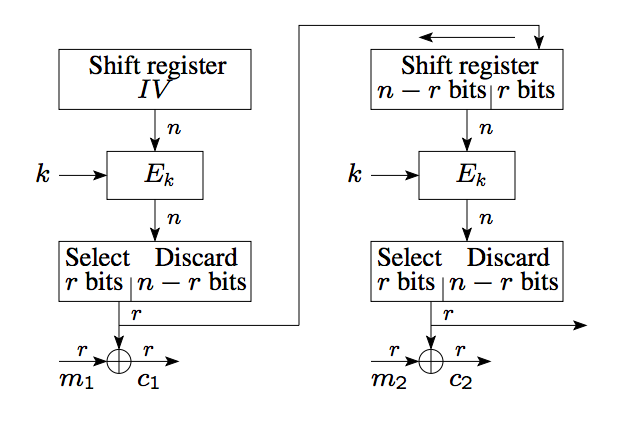
\includegraphics[scale=0.5]{ofb_encryption.png}
\caption{Encryption using Output Feedback Mode \citep{lecture3_marina}}
\label{fig:ofb_encryption}
\end{figure}

Following the same footsteps as CFB we get, $C_1$ = $S_r(E_k(I_1))$ $\oplus$ $m_1$
\newline \newline However, the contents of the shift register are left-shifted left by r bits and the left-most (most significant) r bits of the encrypted output,  $S_r(E_k(I_1))$ is placed in the right-most (least significant) r bits of the shift register i.e $I_2$ = $ (I_1 \ll r) \| S_r(E_k(I_1))$
\newline \newline Generalizing this formula we get,

$C_i$ = $S_r(E_k(I_i))$ $\oplus$ $m_i$ ; $I_{i+1}$ = $ (I_i \ll r) \| S_r(E_k(I_i))$ 
\newline \newline Since the inverse of XOR is XOR only, we can derive the decryption formula from above.

$m_i$ = $S_r(E_k(I_i))$ $\oplus$ $C_i$ ; $I_{i+1}$ = $ (I_i \ll r) \| S_r(E_k(I_i))$ 



\section{Question}

\textbf{Suppose researcher Alice discovers a ground-breaking algorithm for which she thinks the public is not ready. Instead of announcing it, Alice describes the algorithm in a document and publishes a cryptographic hash of it in the current issue of a newspaper. When 15 years later the research community gets close to rediscovering the algorithm, Alice announces the result.}

\textbf{(a) Can the digest published in the newspaper be used as a proof (i.e., convince a judge) that the algorithm was discovered 15 years ago? Justify your answer.}
\newline \newline This is an interesting use-case to consider. To prove that Alice is the original author of the algorithm, besides demonstrating the original draft describing the algorithm, she has to prove that it was originated before the new inventor devised the algorithm.

\begin{enumerate}
\item Though it is a one-way hashing function, so the original plain-text cannot be retrieved from the digest. But one plaintext will always generate the same digest. If she can demonstrate, the original text is generating the same digest which was published in the newspaper, her argument can hardly be refuted.

A counterargument could be made against her case, as we need to consider collisions for hashing functions. But here, though it's mathematically not impossible, it is highly improbable. So this counterargument can be discounted.

\item The newspaper here is practically working as Trusted Timestamping. It was published 15 years ago and as a result, a well-documented and well-circulated case like that cannot be altered.
\end{enumerate}

I believe, she can provide enough information to convince the judge that she is the original inventor of this algorithm.




\newpage \textbf{(b) Would your answer change if a cryptographic signature of the document was published instead of the hash? Justify.}

A digital signature is a mathematical technique used to validate the authenticity and integrity of a message, software or digital document. It is intended to solve the problem of tampering and impersonation in digital communications.

\begin{figure}[h]
\centering
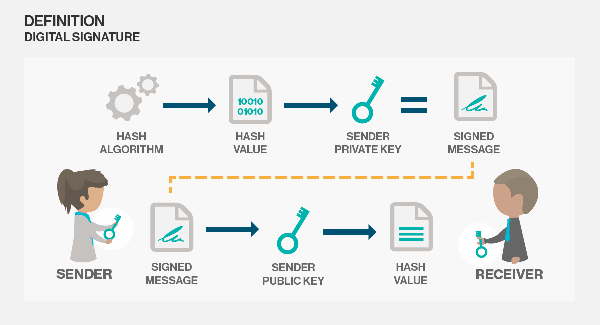
\includegraphics[scale=0.5]{dsig.png}
\caption{How digital signature works \citep{tt_dsig}}
\label{fig:digital_signature}
\end{figure}

In this case Alice already has enough information to prove the authenticity of her claim. Since except her, no one can provide the original text of the digest, there is no question of tampering/impersonating. Though signing the message and conjuring the key pairs provides an extra proof of her identity, the primary purposes of digital signature are already redundant in this case. After decrypting it with the key, we will get the same digest and that leaves us in the same situation as question no 2(a).
\newline \newline So in both cases, she should be able to prove the authenticity of her claim.


\section{Question}

\textbf{Suppose Alice and Bob store their respective RSA encryption public keys in a file on a server. They communicate regularly using confidential messages. Eve wants to read the messages but is unable to crack the RSA private keys of Alice and Bob. However, she is able to break into the server and alter the file containing Alice’s an Bob’s public keys.}
\newline \newline \textbf{(a) How should Eve alter that file so that she can read confidential messages sent between Alice and Bob and forge messages from either? After altering the file, how would she need to modify the communication to achieve the above?}


\begin{figure}[h]
\centering
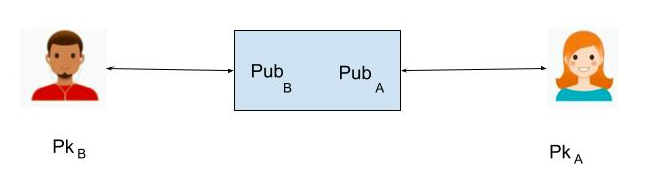
\includegraphics[scale=0.5]{3a.jpg}
\caption{Communication between Bob and Alice}
\label{fig:bob_alice}
\end{figure}

In ideal case:
\begin{enumerate}

\item Bob will encrypt the message using Alice's public key $Pub_A$.
\item Alice will decrypt it using her private key $Pk_A$
\item Alice will encrypt the message using Bob's public key $Pub_B$.
\item Bob will decrypt it using his private key $Pk_B$

\end{enumerate}

\newpage Now since Eve was able to compromise the server, she has both the public keys of Bob and Alice. She can use the Man-in-the-middle attack in this case to intercept, understand and impersonate Alice or Bob.


\begin{figure}[h]
\centering
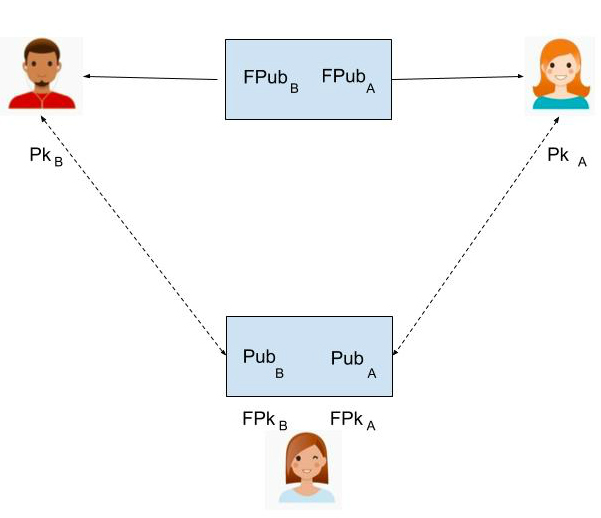
\includegraphics[scale=0.5]{3b.jpg}
\caption{Man-in-the-middle attack executed by Eve}
\label{fig:eve_here}
\end{figure}


\begin{enumerate}

\item Eve will create two new key pairs $FPub_A$ , $FPk_A$ and $FPub_B$ , $FPk_B$
\item She will replace the original public keys $Pub_A$ and $Pub_B$ with $FPub_A$ and $FPub_B$ respectively.
\item Bob will encrypt the message using Eve's public key $FPub_A$.
\item Eve can intercept this message and decrypt it with $FPk_A$. After reading the content she may modify the message if she deems it necessary. Then encrypts it again with $Pub_A$. Then send it to Alice impersonating Bob.
\item Alice will decrypt it using her private key $Pk_A$. She will conclude the message was sent by Bob, unmodified and uninterrupted.


\item Same wat Alice will encrypt the message using Eve's public key $FPub_B$.
\item Eve can intercept this message as well as decrypt it with $FPk_B$. After reading the content she may modify the message if she deems it necessary. Then encrypts it again with $Pub_B$. Then send it to Bob impersonating Alice.
\item Bob will decrypt it using his private key $Pk_B$. He will conclude the message was sent by Alice, unmodified and uninterrupted.

\end{enumerate}



\textbf{(b) How might Alice and/or Bob detect Eve’s subversion of the public keys?}
\newline \newline Once the current communication channel is compromised, there is no way Alice or Bob can discover their conversation is being eavesdropped and messages are getting altered. They can change the method of communication channel if they suspect this happening.

But what they should have done are adding security measures to prevent this scenario. They have to make sure that, both of them  are using the correct public key. In this case, they could have Alice and Bob's public keys be distributed as certificates, signed by a trusted third party, let's call him Trent. Trent's public key is known to everybody ahead of time (eg. distributed with the software), and the server does not know Trent's private key, so Even cannot forge certificates.

This system can be strengthen many folds by introducing more trusted third parties. In cryptography, it is called Web of trust.

\newpage
\textit{
    In cryptography, a web of trust is a concept used in PGP, GnuPG, and other OpenPGP-compatible systems to establish the authenticity of the binding between a public key and its owner. Its decentralized trust model is an alternative to the centralized trust model of a public key infrastructure (PKI), which relies exclusively on a certificate authority (or a hierarchy of such). As with computer networks, there are many independent webs of trust, and any user (through their identity certificate) can be a part of, and a link between, multiple webs. 
}\citep{wot_wiki}

\begin{figure}[h]
\centering
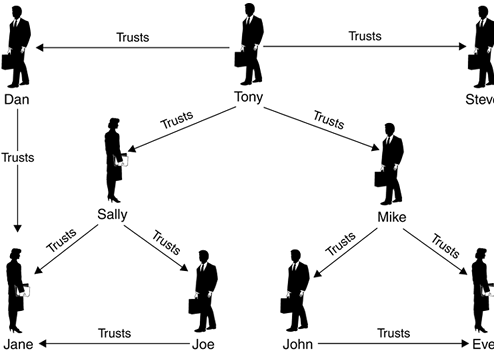
\includegraphics[scale=0.5]{wot.png}
\caption{An illustration for Web on Trust Model \citep{butebanwot}}
\label{fig:wot}
\end{figure}



\section{Question}

\textbf{
Read the paper “Why Cryptosystems Fail” (available from http://www.buffalo.edu/\~mblanton/cse565/wcf.pdf) and answer the following questions about it:}
\newline \newline \textbf{(a) What does the article tell you about security of computer systems and how the field of security evolves?}
\newline \newline The article describes a time in history, more specifically in the 1970's, when an industry-wide threat model was adopted. As till that time only military organizations worked with information security, the industry tried to take advantage of their wisdom. As military model stressed secrecy, it was an assumption that the information leak will not happen in a civilian environment, and the clients will be able to hire people with significant training and expertise to implement these threat models. As it turned out, this is completely irrelevant as required efficiency, secrecy and competency cannot be expected in practical scenarios.
\newline \newline This philosophy may work in a controlled environment but once the scaling increased it becomes a bottleneck. It's not possible to control so many involved people to maintain the integrity of the system. For example, one bank clerk in Hastings branch was able to withdraw money from a housewife's account. He was even able to conceal the withdrawal transactions to appear in bank statements.
\newline \newline At the beginning the banks tried to devise their own algorithms and implement it. But since there are thousands of banks, as expected most of them have failed to put an effective and secure system. 
\newline \newline With the rise of new standardized algorithms, banks started implementing them. But due to the lack of proper security expert, management's stand on prioritizing convenience before security did not yield a positive result. For example, a four digit pin can have 9999 combinations. If three attempts are allowed there is 1/3333 chance for the adversary to get it right. The bank suggested their client to use a distinctive piece of squared cardboard to remember the pin which in turn make the odds of getting it right in 1 out of 8 chances.
\newline \newline Integrating with security product providers like Visa/Mastercard was another attempt to provide the informational integrity and prevent fraud. Banks tried to adhere to guidelines provided by these security module providers but even this was not foolproof. There was an incident where an emulation software packages were set to log all
the transactions passing through. The contractor captured the clear zone
key as it was created, and later used it to decrypt the bank’s PIN key.
\newline \newline From the evolution of bank security described above we can understand, though progress has been made in computer security, there is something inherently wrong in the underlying philosophy. That is the reason why we are not able to reach the perfection described in theoretic design in the practical world. That is why the author proposed, the security research models needs a new paradigm shift. 
\newline \newline  \textbf{(b) What does it tell you about building and operating secure systems?}
\newline \newline Building and operating secure system can be a tricky job, as there are infinite number of scenarios might happen which will cause the system to be compromised. 

\begin{enumerate}

\item Government should pass a law so that companies cannot make their consumers scrap-goats in case of security violation and they will be held responsible to maintain a secure system.

\item A management which is willing to prioritize integrity and security over convenience needs to be instilled.

\item A team of full-time security experts with irrefutable reputation needs to be hired, who has to expertise to implement at least the standard security systems perfectly. Cost and resource should not be a problem when the design and implementation of the security is concerned.

\item Proper guidelines should be designed for the people who are going to be conducting the day-to-day operation. The fail-safes should be put places so that if any unforeseen incident occurs, it can be remedied. Companies must ensure policies and guidelines are being followed.

\item Processes should be automated as much as possible. The fewer people are involved, fewer security risks are there.

\item Every action has to be audited. Non-repudiation measures should be implemented everywhere to maintain the integrity of the system.

\end{enumerate}
\newline \newline \textbf{(c) What is the main proposal of the paper?}
\newline \newline The author argues the design philosophy of the security experts is completely wrong. Whereas the security equipment designers and government evaluators have both concentrated on technical weaknesses,
such as poor encryption algorithms and operating systems, the real threat is the poor implementation of these standards, lack of expertise, an indifferent attitude from the administration.
\newline \newline His main proposal is, the security community should adopt a new philosophy. Instead of keeping secrets of the failings, the community should collaborate in this and together the advancement in designing a perfect security system will be much faster, as the entities do not have to make the same mistakes and re-invent the wheel again and again. He proposed, instead of worrying about what might possibly go wrong, we need to make a systematic study of what is likely to; Each and every process needs to be monitored closely, and proper quality control measures should be implemented in each step.
\newline \newline The author suggested like it's predecessors in other fields when a paradigm shift occurs, it is quite common for a research model to be imported from some other discipline in order to give structure to the newly emerging results. He deems the research models for safety-critical system worthy of following. He, in fact, suggested two approaches from critical system industry; First one follows the reductionist design philosophy, which is the implementation of a railway signaling system. The second one is more holistic, the aviation paradigm is based on constant top-level feedback and incremental improvement.  
\newline \newline \textbf{(d) How do you think the situation with the banking industry today compares with what is described in the article? What are some of the protection mechanisms that you encountered in your banking experience?}
\newline \newline Security in today's banking system has developed greatly. In fact, the security world has implemented some of the ideas the author has hinted in this article, which proves phenomenal vision on his part. Most of the security incidents he mentioned are trivial now.
\newline \newline With the rise of cloud everything is integrated all the time. Most of the common anomalies trigger the security system within a split second of happening. The extensive security systems have been adopted in other industries as well. So besides open-source communities, even companies are sharing the use cases where their security system failed to prevent an attack. Unforeseen events are getting reported every day, security experts now have enough information to work on problems.
\newline \newline Most of the processes are either automated or the work that requires manual intervention, those are closely monitored.
\newline \newline As a consumer, I have come across different security measures whenever I use banking services. For example: 

\begin{enumerate}
\item \textbf{Two-factor Authentication}: Before completing the transaction One Time Password is generated and sent as SMS/email to verify that owner of the account are doing that transaction.

\item \textbf{Notification}: If the balance is deducted from our bank account, we get an instant notification stating information, where, how much or to whom the money has been paid.

\item \textbf{Obscurification}:  Account number is an important detail that should not be shared lightly. A few years ago, the Indian Government implemented Unified Payment Interface (UPI), a real-time payment system facilitating inter-bank transactions. This way, to send money sender do not need to know the bank account number of the receiver. A unique identifier like the phone number can be used to complete bank transfers.

\item \textbf{Cross Confirmation}: Banks keep track of our spending habits. If a transaction has been made, which does not align with consumer's spending pattern an automatic confirmation call is triggered, which takes the customer's consent again to validate the authenticity of the transaction.

\item \textbf{Password Regeneration}: In every few months the netbanking account forces the user to set a strong new password to prevent account compromisation events.
\end{enumerate}
\newline \newline \textbf{(e) How do you think computer security in other industries compares to the security in the banking sector?}
\newline \newilne In this information age, it has become a prime concern for all the industries to safe guard their information. Though banking and finance industry have been the pioneer in in security implementation, others are trying to catch up with it, as their information proved as valuable. Here is the  list of arguably the top 5 most attacked Industries in recent years.
\newline \newline \textbf{Healthcare}: An industry full of confidential information and a prime target for hackers. Hospitals have access to electronic healthcare records, containing large amounts of information, from names and addresses of patients to their physical condition and financial details. The recent WannaCry ransom-ware attack left devastating effects in multiple hospitals all over the world impacting patient care. As can be guessed, not all the health care centers has the same level sophisticated security system, as a result an easy target for hackers.
\newline \newline \textbf{Manufacturing}: This industry includes automotive, electronics, and pharmaceutical companies, affects the day-to-day life of average consumer. Most of the attackers are financially motivated and therefore are more likely to hack corporations where they can demand a higher amount of money, as well as sell information to competitors. Intellectual property is also incredibly valuable and so attackers may also be after that. But comparatively, when it comes to security compliance and risk management, manufacturing sector does not put the same effort as Financial sector.
\newline \newline \textbf{Education}: Education institutions are gold mines for cyber attackers. Not only they have valuable student information, government identifications, the universities has access to high end hardware resources which can be used to mount attack on other industries. Universities also has repository of confidential and cutting edge research material. Main stream universities take security violations seriously, but situations of most of education institutions are abysmal.
\newline \newline \textbf{Legal Sector}: Law firms are a soft target for cyber attackers. This sector has information about all other industries as they are the their clients. Sensitive information such as patent and litigation information, financial data, and upcoming merger and acquisition documents etc. Most of the law firms lacks sophisticated cyber security defence. So if any cyber attack was thwarted by the company, attacker concentrate on the law firms serving them to extract information.
\newline \newline \textbf{Government}: Historically, attackers have always attacked governments institutions. In 2015, millions of U.S. employee records including social security numbers, birthplace and digitized employee fingerprints were exposed. Over 50 million Turkish citizens were at risk of identity theft and over a million Japanese citizens were exposed due to the opening of a malicious email attachment by the pension service. Though the military institutions are quite adept in defending their information, other institutions are not that competent, this happens due to the scale the government works at.

It can be concluded that, financial industries are still one of the forerunner in implementing security.


\nocite{globsi}
\nocite{compsec_wl}
\bibliographystyle{unsrt}
\bibliography{references}
\end{document}
